\section{Introduction}

\begin{frame}

	\begin{itemize}[<+->]
		\item L'apparition d'un ordinateur central capable d'effectuer des opérations complexes
		\item Initié dans le domaine de la \textbf{recherche} et adopté par \textbf{le gouvernement}.
		\item Plus tard, son utilisation s'est étendue aux \textbf{entreprises}.
	\end{itemize}

\end{frame}

\begin{frame}

	\begin{itemize}[<+->]
			\item La nécessité d'un périphérique capable d'envoyer des instructions et de recevoir une réponse était cruciale à l'époque

			\item Un périphérique physique était souvent connecté à l'unité centrale via un port série, tel que \textbf{COM1}

				\begin{figure}
					\centering
					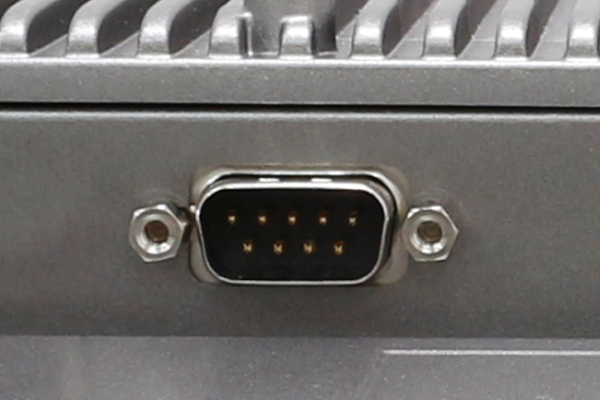
\includegraphics[width=3cm]{images/com1_serial.jpg}
					\caption{Un port série COM1}
				\end{figure}

			\item À cette époque, un ordinateur central était considéré comme un \textit{"réseau de terminaux"}
	\end{itemize}


\end{frame}

\begin{frame}

	\begin{itemize}[<+->]
		\item Le périphérique physique utilisé à l'époque était communément appelé un \textbf{terminal}.
		\item Un exemple bien connu de terminal physique était le \textbf{VT100}.

			\begin{figure}
				\centering
				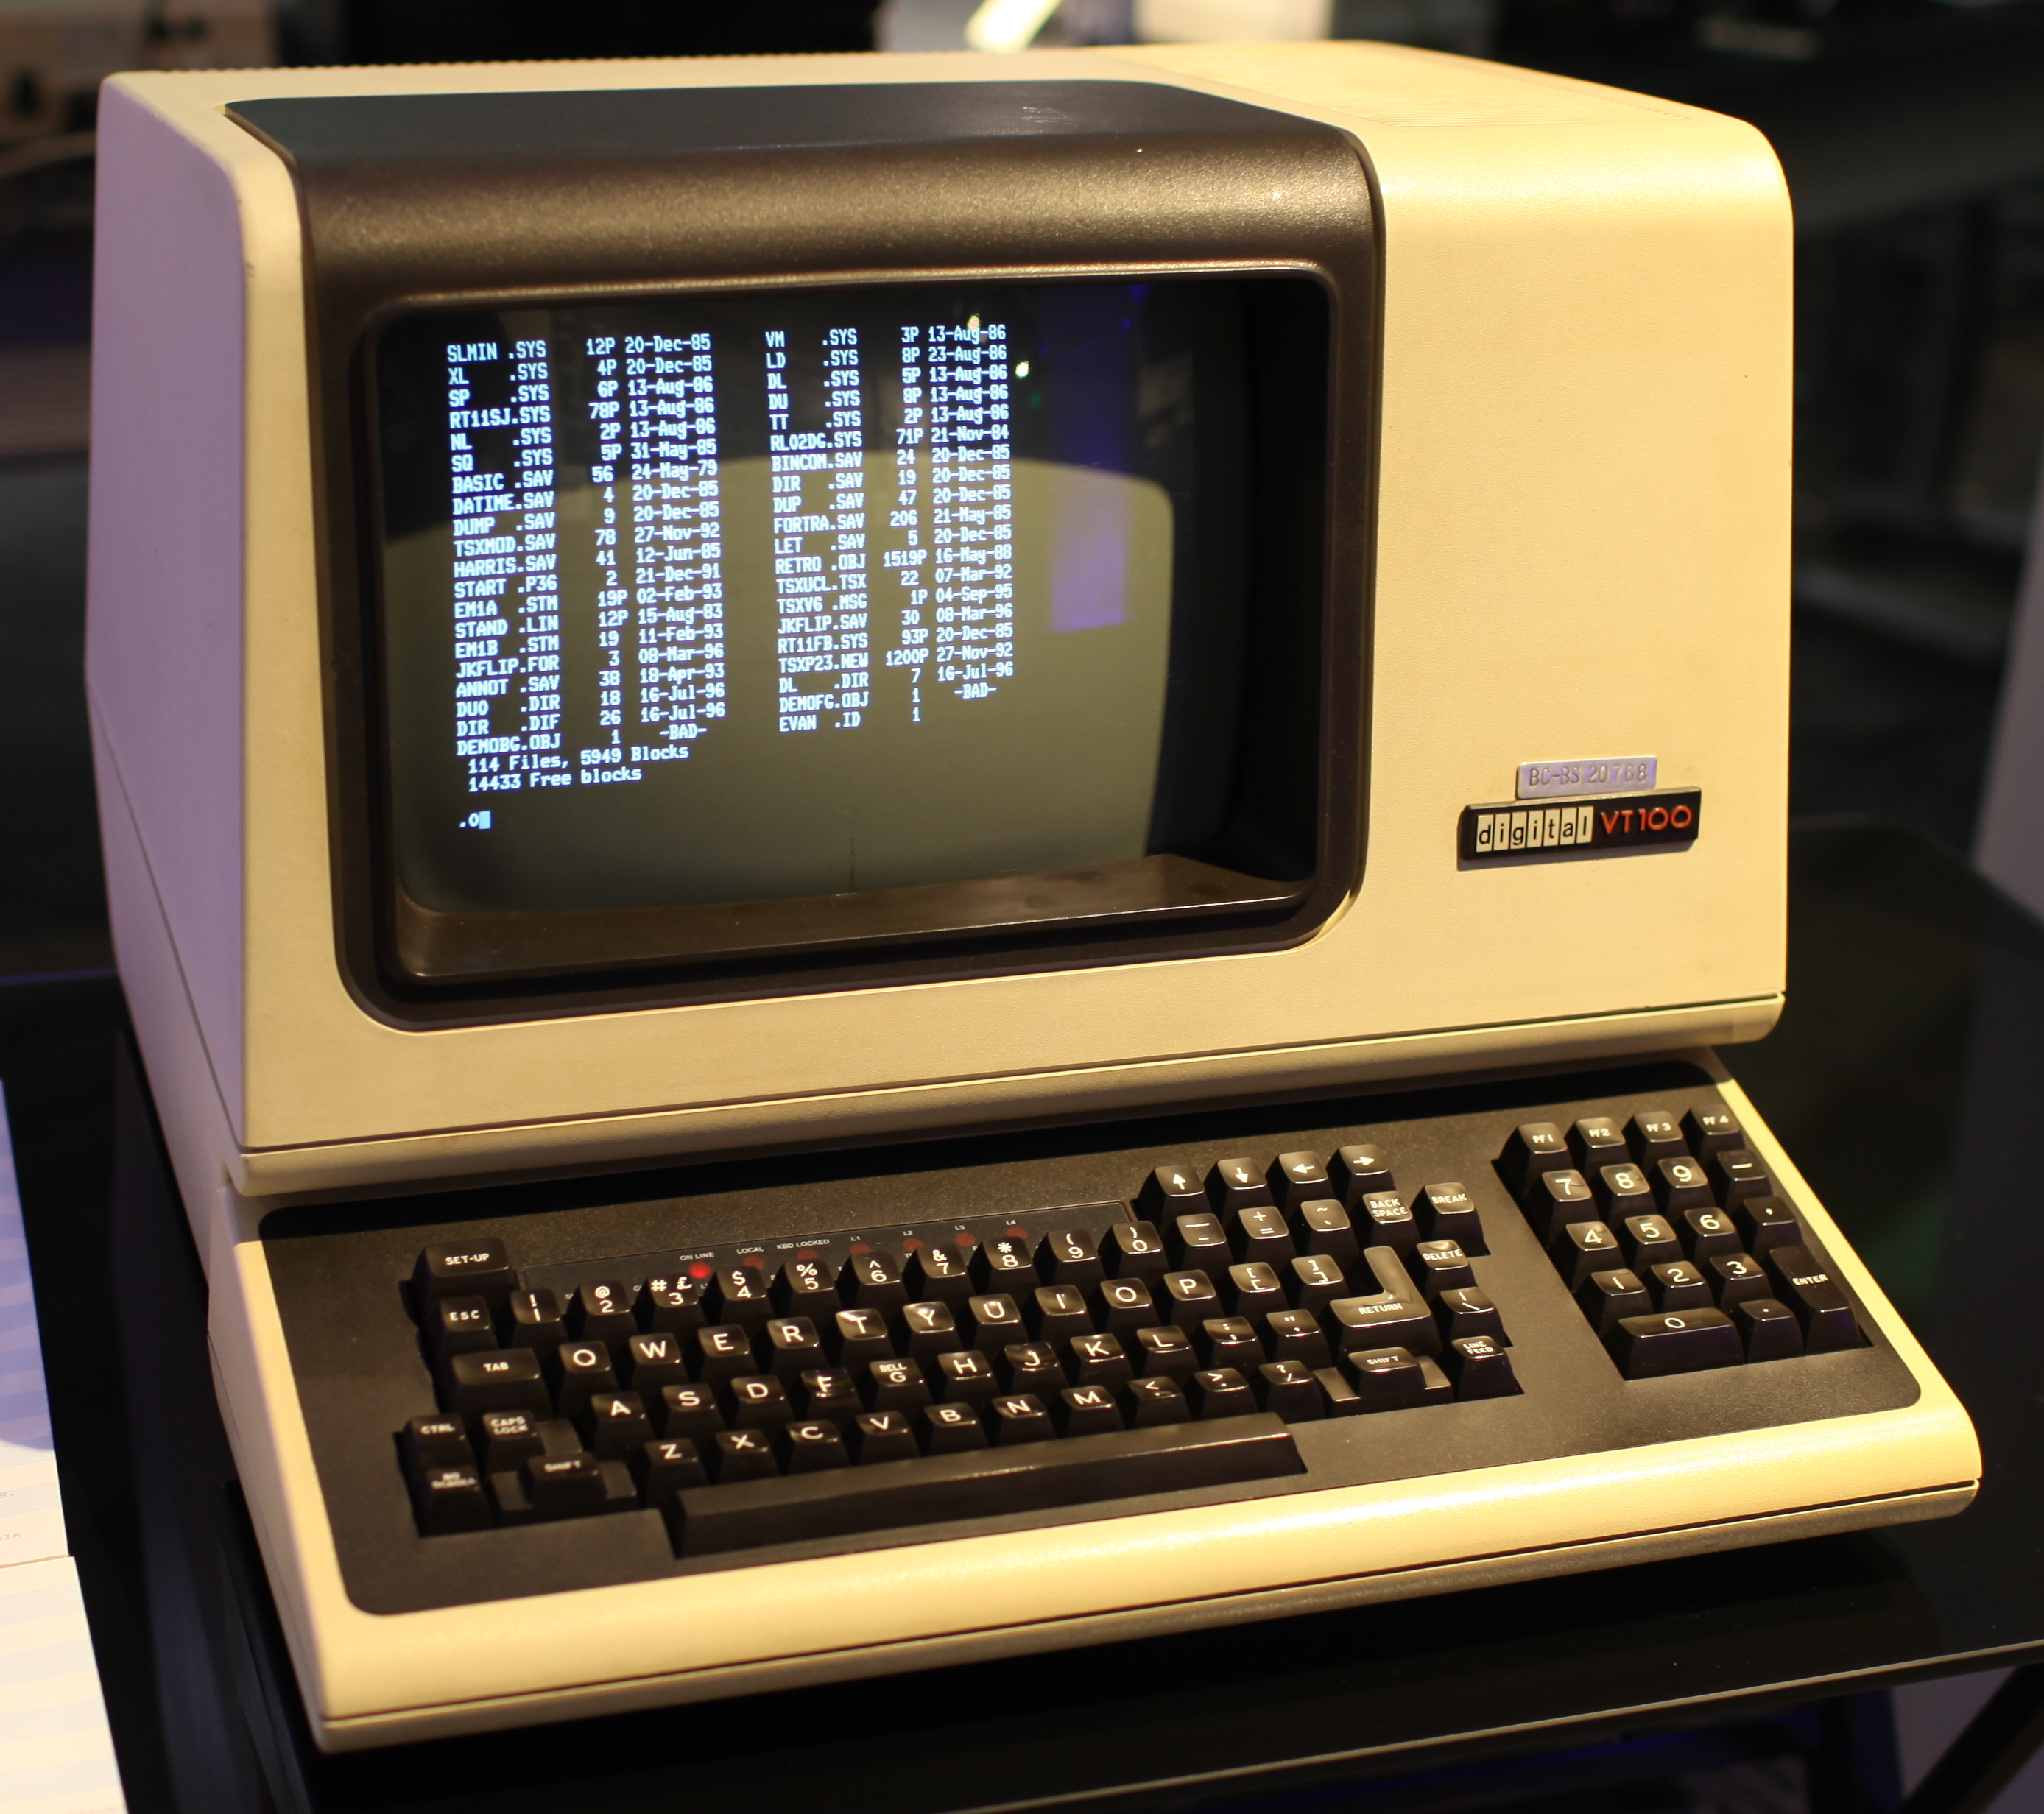
\includegraphics[width=4cm]{images/DEC_VT100_terminal.jpg}
				\caption{Un terminal physique DEC VT100 avec écran et clavier.}
			\end{figure}

		\item Les utilisateurs pouvaient accéder aux ressources de l'unité centrale à partir du terminal physique.
	\end{itemize}

\end{frame}
